% Options for packages loaded elsewhere
\PassOptionsToPackage{unicode}{hyperref}
\PassOptionsToPackage{hyphens}{url}
\PassOptionsToPackage{dvipsnames,svgnames,x11names}{xcolor}
%
\documentclass[
  10pt,
  a4paper,
  DIV=11]{scrartcl}

\usepackage{amsmath,amssymb}
\usepackage{iftex}
\ifPDFTeX
  \usepackage[T1]{fontenc}
  \usepackage[utf8]{inputenc}
  \usepackage{textcomp} % provide euro and other symbols
\else % if luatex or xetex
  \usepackage{unicode-math}
  \defaultfontfeatures{Scale=MatchLowercase}
  \defaultfontfeatures[\rmfamily]{Ligatures=TeX,Scale=1}
\fi
\usepackage{lmodern}
\ifPDFTeX\else  
    % xetex/luatex font selection
  \setmainfont[]{Arial}
\fi
% Use upquote if available, for straight quotes in verbatim environments
\IfFileExists{upquote.sty}{\usepackage{upquote}}{}
\IfFileExists{microtype.sty}{% use microtype if available
  \usepackage[]{microtype}
  \UseMicrotypeSet[protrusion]{basicmath} % disable protrusion for tt fonts
}{}
\makeatletter
\@ifundefined{KOMAClassName}{% if non-KOMA class
  \IfFileExists{parskip.sty}{%
    \usepackage{parskip}
  }{% else
    \setlength{\parindent}{0pt}
    \setlength{\parskip}{6pt plus 2pt minus 1pt}}
}{% if KOMA class
  \KOMAoptions{parskip=half}}
\makeatother
\usepackage{xcolor}
\usepackage[top=30mm,left=20mm,heightrounded]{geometry}
\setlength{\emergencystretch}{3em} % prevent overfull lines
\setcounter{secnumdepth}{3}
% Make \paragraph and \subparagraph free-standing
\ifx\paragraph\undefined\else
  \let\oldparagraph\paragraph
  \renewcommand{\paragraph}[1]{\oldparagraph{#1}\mbox{}}
\fi
\ifx\subparagraph\undefined\else
  \let\oldsubparagraph\subparagraph
  \renewcommand{\subparagraph}[1]{\oldsubparagraph{#1}\mbox{}}
\fi


\providecommand{\tightlist}{%
  \setlength{\itemsep}{0pt}\setlength{\parskip}{0pt}}\usepackage{longtable,booktabs,array}
\usepackage{calc} % for calculating minipage widths
% Correct order of tables after \paragraph or \subparagraph
\usepackage{etoolbox}
\makeatletter
\patchcmd\longtable{\par}{\if@noskipsec\mbox{}\fi\par}{}{}
\makeatother
% Allow footnotes in longtable head/foot
\IfFileExists{footnotehyper.sty}{\usepackage{footnotehyper}}{\usepackage{footnote}}
\makesavenoteenv{longtable}
\usepackage{graphicx}
\makeatletter
\def\maxwidth{\ifdim\Gin@nat@width>\linewidth\linewidth\else\Gin@nat@width\fi}
\def\maxheight{\ifdim\Gin@nat@height>\textheight\textheight\else\Gin@nat@height\fi}
\makeatother
% Scale images if necessary, so that they will not overflow the page
% margins by default, and it is still possible to overwrite the defaults
% using explicit options in \includegraphics[width, height, ...]{}
\setkeys{Gin}{width=\maxwidth,height=\maxheight,keepaspectratio}
% Set default figure placement to htbp
\makeatletter
\def\fps@figure{htbp}
\makeatother

%% load packages
\usepackage{sectsty}
\usepackage{fontspec}
\usepackage{scrlayer-scrpage}
\usepackage{fontspec}

% Define title formatting

%% Set font sizes for sections and subsections
\sectionfont{\fontsize{11}{16}\selectfont\bfseries} % Arial 14pt bold
\subsectionfont{\fontsize{10}{14}\selectfont} % Arial 12pt

\lehead[test1]{\pagemark}
\cehead[]{}
\rehead[test 2]{\leftmark}
\lohead[{\fontsize{8}{10}\selectfont\upshape\textbf{Institut Sekundarstufe I}} \\
\fontsize{8}{10}\selectfont\upshape Fabrikstrasse 8, CH-3012 Bern \\
\fontsize{8}{10}\selectfont\upshape T +41 31 309 21 15, contactdesk@phbern.ch, www.phbern.ch
]{\rightmark}
\rohead[PHBern]{}
\KOMAoption{captions}{tableheading}
\makeatletter
\@ifpackageloaded{tcolorbox}{}{\usepackage[skins,breakable]{tcolorbox}}
\@ifpackageloaded{fontawesome5}{}{\usepackage{fontawesome5}}
\definecolor{quarto-callout-color}{HTML}{909090}
\definecolor{quarto-callout-note-color}{HTML}{0758E5}
\definecolor{quarto-callout-important-color}{HTML}{CC1914}
\definecolor{quarto-callout-warning-color}{HTML}{EB9113}
\definecolor{quarto-callout-tip-color}{HTML}{00A047}
\definecolor{quarto-callout-caution-color}{HTML}{FC5300}
\definecolor{quarto-callout-color-frame}{HTML}{acacac}
\definecolor{quarto-callout-note-color-frame}{HTML}{4582ec}
\definecolor{quarto-callout-important-color-frame}{HTML}{d9534f}
\definecolor{quarto-callout-warning-color-frame}{HTML}{f0ad4e}
\definecolor{quarto-callout-tip-color-frame}{HTML}{02b875}
\definecolor{quarto-callout-caution-color-frame}{HTML}{fd7e14}
\makeatother
\makeatletter
\@ifpackageloaded{caption}{}{\usepackage{caption}}
\AtBeginDocument{%
\ifdefined\contentsname
  \renewcommand*\contentsname{Inhaltsverzeichnis}
\else
  \newcommand\contentsname{Inhaltsverzeichnis}
\fi
\ifdefined\listfigurename
  \renewcommand*\listfigurename{Abbildungsverzeichnis}
\else
  \newcommand\listfigurename{Abbildungsverzeichnis}
\fi
\ifdefined\listtablename
  \renewcommand*\listtablename{Tabellenverzeichnis}
\else
  \newcommand\listtablename{Tabellenverzeichnis}
\fi
\ifdefined\figurename
  \renewcommand*\figurename{Abbildung}
\else
  \newcommand\figurename{Abbildung}
\fi
\ifdefined\tablename
  \renewcommand*\tablename{Tabelle}
\else
  \newcommand\tablename{Tabelle}
\fi
}
\@ifpackageloaded{float}{}{\usepackage{float}}
\floatstyle{ruled}
\@ifundefined{c@chapter}{\newfloat{codelisting}{h}{lop}}{\newfloat{codelisting}{h}{lop}[chapter]}
\floatname{codelisting}{Listing}
\newcommand*\listoflistings{\listof{codelisting}{Listingverzeichnis}}
\makeatother
\makeatletter
\makeatother
\makeatletter
\@ifpackageloaded{caption}{}{\usepackage{caption}}
\@ifpackageloaded{subcaption}{}{\usepackage{subcaption}}
\makeatother
\ifLuaTeX
\usepackage[bidi=basic]{babel}
\else
\usepackage[bidi=default]{babel}
\fi
\babelprovide[main,import]{ngerman}
\ifPDFTeX
\else
\babelfont{rm}[]{Arial}
\fi
% get rid of language-specific shorthands (see #6817):
\let\LanguageShortHands\languageshorthands
\def\languageshorthands#1{}
\ifLuaTeX
  \usepackage{selnolig}  % disable illegal ligatures
\fi
\usepackage{bookmark}

\IfFileExists{xurl.sty}{\usepackage{xurl}}{} % add URL line breaks if available
\urlstyle{same} % disable monospaced font for URLs
\hypersetup{
  pdftitle={Theoretische Grundlagen},
  pdfauthor={Richard Conrardy},
  pdflang={de},
  colorlinks=true,
  linkcolor={(3,1.5)},
  filecolor={Maroon},
  citecolor={Blue},
  urlcolor={Blue},
  pdfcreator={LaTeX via pandoc}}

\title{Theoretische Grundlagen}
\usepackage{etoolbox}
\makeatletter
\providecommand{\subtitle}[1]{% add subtitle to \maketitle
  \apptocmd{\@title}{\par {\large #1 \par}}{}{}
}
\makeatother
\subtitle{Grundlagen der Beurteilung}
\author{Aline Löw \and Daniel Ingrisani \and Irene Althaus}
\date{01.01.2024}

\begin{document}
\maketitle
\begin{abstract}
Mit diesem Lernmodul erhalten Sie nicht bloss eine Einführung in die
Thematik «Beurteilung und Förderung», sondern auch ein Grundgerüst an
Begriffsdefinitionen, die für das Verständnis und die Begründung der
eigenen Beurteilungspraxis von entscheidender Bedeutung sind.
\end{abstract}

\begin{tcolorbox}[enhanced jigsaw, leftrule=.75mm, title=\textcolor{quarto-callout-note-color}{\faInfo}\hspace{0.5em}{Ziele des Lernmoduls}, toprule=.15mm, breakable, toptitle=1mm, rightrule=.15mm, opacitybacktitle=0.6, opacityback=0, colback=white, colbacktitle=quarto-callout-note-color!10!white, bottomtitle=1mm, titlerule=0mm, colframe=quarto-callout-note-color-frame, arc=.35mm, bottomrule=.15mm, left=2mm, coltitle=black]

Die Studierenden \ldots{}

\begin{itemize}
\tightlist
\item
  kennen die Bedeutung von «beurteilen» und «fördern» und können beides
  voneinander unterscheiden.
\item
  kennen die Begriffe «formativ» und «summativ» und können diese im
  Lernen der SuS verorten.
\item
  erkennen, dass sowohl das Beurteilen als vor allem auch das Fördern
  Kreisprozesse darstellen, die auch in Kreisläufen dargestellt werden
  können.
\item
  erarbeiten sich eine differenzierte Sicht des Begriffs der «Leistung»
  und damit auch der «Leistungsbeurteilung».
\item
  entwickeln ein Bewusstsein für die Komplexität von Beurteilung \&
  Förderung, indem Sie das sowohl widersprüchliche als auch harmonische
  Zusammenspiel zwischen Gerechtigkeit, Bezugsnormen und
  Beurteilungsfunktionen erfassen.
\end{itemize}

\end{tcolorbox}

\section{1. Input zur Einführung}\label{input-zur-einfuxfchrung}

Mit Abbildung~\ref{fig-screencast} erhalten Sie eine Einführung in die
Thematik und Sie lernen die Unterscheidung zwischen «summativer» und
«formativer» Beurteilung kennen.

\begin{figure}

\centering{

}

\caption{\label{fig-screencast}Screencast zur formativen und summativen
Beurteilung}

\end{figure}%

\section{2. Input Kreisläufe}\label{input-kreisluxe4ufe}

Im Wissen darum, dass sowohl das Beurteilen als vor allem auch das
Fördern in Kreisprozessen ablaufen, stellen wir Ihnen in diesem Input
einen \textbf{Förderkreislauf} sowie zwei stärker auf die Beurteilung
ausgerichtete \textbf{Beurteilungskreisläufe} vor.

Solche Kreismodelle sollen einerseits ermöglichen die Komplexität der
Thematik überschaubar zu halten und zudem helfen, aufeinander aufbauende
Aspekte der Beurteilung und Förderung besser zu verstehen. Es lohnt sich
deshalb auch für das eigene Beurteilungskonzept sich von solchen
Modellen leiten zu lassen. Allenfalls entwickeln Sie darauf aufbauend
ein eigenes Kreismodell Ihres persönlichen Beurteilungskonzeptes.

\subsubsection{Beurteilung im Kanton
Bern}\label{beurteilung-im-kanton-bern}

Ein spezielles Augenmerk möchten wir auf die Beurteilungssituation im
Kanton Bern richten. Im Input werden wir abschliessend auch den unten
abgebildeten Kreislauf vorstellen, wo sowohl das Vokabular, als auch die
gesetzlichen Vorgaben des Kantons schematisch abgebildet sind. Innerhalb
der beiden Beurteilungsmodulen (Formative und Summative, prognostische
Beurteilung) haben sich die Dozierenden darauf geeinigt, dass wir uns im
Sinne der Kohärenz und des Konsenses vor allem auf diesen Kreislauf
stützen werden. Es lohnt sich deshalb für Sie, diesen kennen zu lernen.
Wie bereits erwähnt, stellen wir Ihnen auch diesen Kreislauf im unten
angefügten Input nächer vor.

\begin{figure}

\centering{

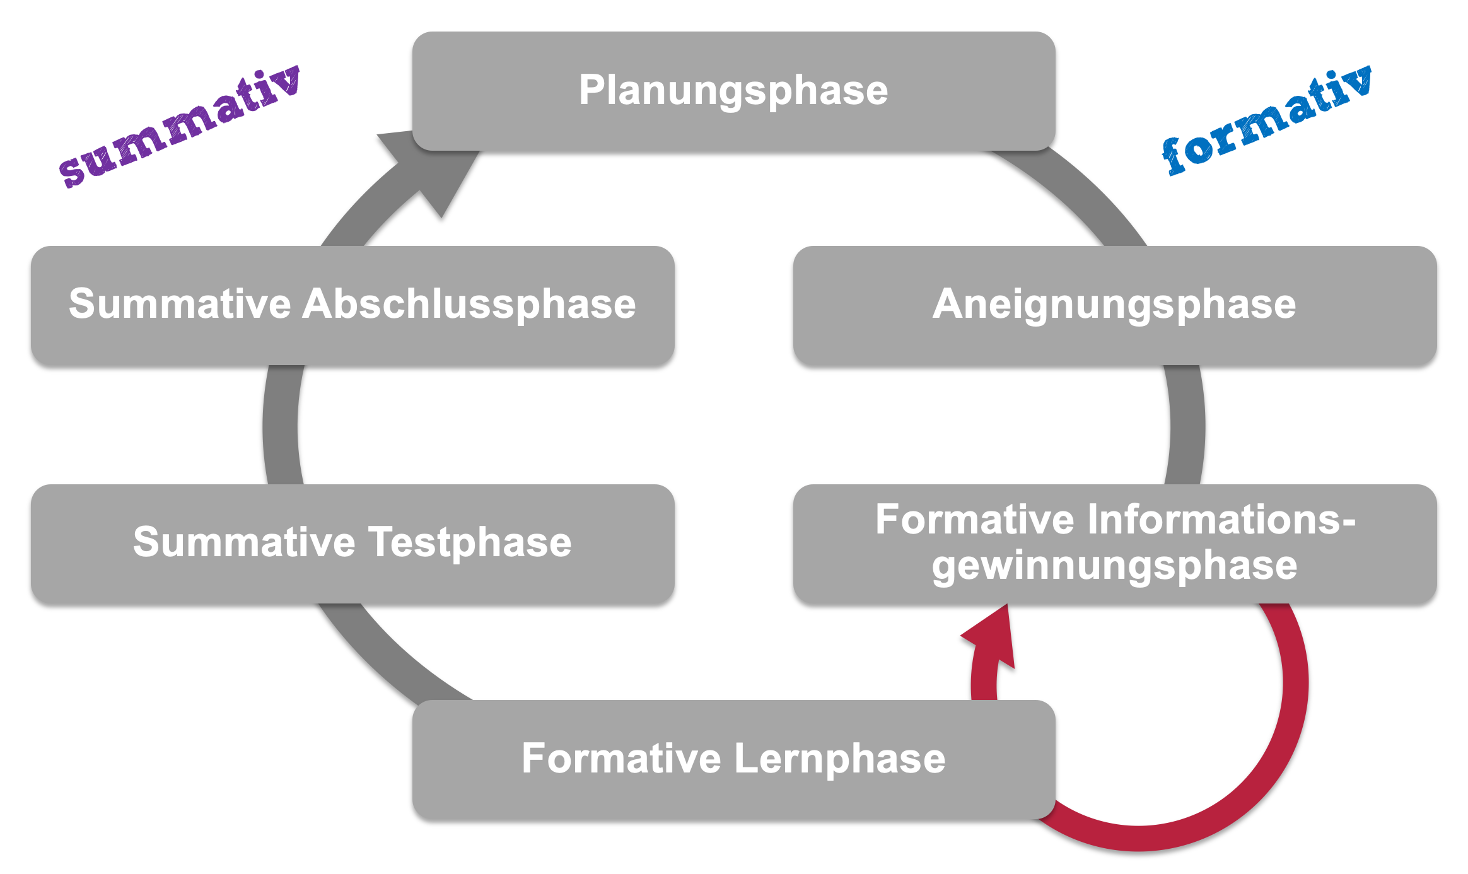
\includegraphics{images/Beurteilungskreislauf_Ingrisani.png}

}

\caption{\label{fig-bild}Förderkreislauf}

\end{figure}%

\begin{figure}

\centering{

}

\caption{\label{fig-förderkreislauf}Screencast zum Förderkreislauf}

\end{figure}%

\subsection{Vertiefung
«Abschlussphase»}\label{vertiefung-abschlussphase}

Wie im Input zu den «Kreisläufen» und dort in den Ausführungen zum
«Beurteilungskreislauf» bereits hingewiesen, stellt die Rückgabe von
Lernkontrollen, Tests oder Prüfungen (gemeint ist die \textbf{summative
Abschlussphase}) ein eher marginalisiertes Thema dar.

Es stellen sich dabei unter anderem folgende Fragen:

\begin{itemize}
\tightlist
\item
  Wie gebe ich den Test zurück? Mit welchen Worten, mit welchen
  Hinweisen?
\item
  Welche Angaben machen Sie auf Ihren Tests (Punkte, Punktedurchschnitt,
  Noten, Notendurchnitt, \ldots)?
\item
  Was ist mit den «Fehlern» oder den «Unkorrektheiten» die in den Tests
  gemacht wurden bzw. mit den «Punkten», die im Test nicht «geholt»
  wurden?
\item
  Werden die Aufgaben noch einmal besprochen? Wenn ja, mit der ganzen
  Klasse oder nur mit einzelnen?
\item
  Muss man den Test «verbessern»? Darf man nachträglich noch zeigen,
  dass man es eingentlich «kann» (Stichwort: Wiederholungstests)?
\end{itemize}

\begin{tcolorbox}[enhanced jigsaw, leftrule=.75mm, title=\textcolor{quarto-callout-caution-color}{\faFire}\hspace{0.5em}{Auftrag auf LearningView}, toprule=.15mm, breakable, toptitle=1mm, rightrule=.15mm, opacitybacktitle=0.6, opacityback=0, colback=white, colbacktitle=quarto-callout-caution-color!10!white, bottomtitle=1mm, titlerule=0mm, colframe=quarto-callout-caution-color-frame, arc=.35mm, bottomrule=.15mm, left=2mm, coltitle=black]

\subsubsection{Auftrag:}\label{auftrag}

Im
\href{https://phbern365.sharepoint.com/:v:/r/sites/IS1.Z.Studienplanentwicklung2022/Freigegebene\%20Dokumente/General/BA\%20-\%20Beurteilung\%20(formativ\%20und\%20summativ)/Lerngelegenheiten/Grundlagen\%20der\%20Beurteilung\%20SOL\%20-\%20Conrardy/Alcala,\%20Leah\%202015\%20-\%20Tch\%20TeachingChannal\%20-\%20Highlighting\%20Mistakes\%20-\%20A\%20Grading\%20Strategy.mp4?csf=1&web=1&e=opTUxg}{folgenden
Video} stellt Ihnen
\href{https://learn.teachingchannel.com/video/math-test-grading-tips}{Alcala,
Leah 2015} von der «Martin Luther King Middle School» in Berkeley (USA)
Ihre «Strategie» vor, wie Sie bei Ihren SuS des 7. und 8. Schuljahres
Tests zurückgibt.

\begin{itemize}
\tightlist
\item
  Lassen Sie sich von diesem «System», von dieser «Strategie» oder von
  dieser Möglichkeit inspirieren und erarbeiten Sie sich Ihre eigenen
  Ideen, Möglichkeiten oder auch schon Strategien.
\item
  Bauen Sie diese schliesslich auch in Ihr Beurteilungskonzept ein.
\end{itemize}

Spannende Aussagen in diesem Video:

\begin{quote}
«So I see that now when I give tests back they're continuing to learn.»
\end{quote}

\begin{quote}
«My hope is, that trough this strategy they see, that studying their
mistakes and learning from their mistakes is really what learning is.»
\end{quote}

Vorschlag für das Bibliografieren und Zitieren des Videos: Alcala, Leah
2015 - Tch TeachingChannal - Highlighting Mistakes - A Grading Strategy

\end{tcolorbox}

\section{3. Input zum
Leistungsbegriff}\label{input-zum-leistungsbegriff}

Wenn es ja «Leistungen» sein sollen, die gefördert und beurteilt werden
sollen, dann ist es unerlässlich, sich im Rahmen des folgenden
Screencasts über den Begriff der schulischen «Leistung» Gedanken zu
machen.

\begin{figure}

\centering{

}

\caption{\label{fig-Leistung}Screencast zum Leistungsbegriff}

\end{figure}%



\end{document}
